\documentclass[11pt]{article}

% Preamble

\usepackage[margin=1in]{geometry}
\usepackage{amsfonts, amsmath, amssymb}
\usepackage{fancyhdr, float, graphicx}
\usepackage[utf8]{inputenc} % Required for inputting international characters
\usepackage[T1]{fontenc} % Output font encoding for international characters
\usepackage{fouriernc} % Use the New Century Schoolbook font
\usepackage[nottoc, notlot, notlof]{tocbibind}
\usepackage{listings}
\usepackage{xcolor}

\definecolor{codegreen}{rgb}{0,0.6,0}
\definecolor{codegray}{rgb}{0.5,0.5,0.5}
\definecolor{codepurple}{rgb}{0.58,0,0.82}
\definecolor{backcolour}{rgb}{0.95,0.95,0.92}

\lstdefinestyle{mystyle}{
    backgroundcolor=\color{backcolour},   
    commentstyle=\color{codegreen},
    keywordstyle=\color{magenta},
    numberstyle=\tiny\color{codegray},
    stringstyle=\color{codepurple},
    basicstyle=\ttfamily\footnotesize,
    breakatwhitespace=false,         
    breaklines=true,                 
    captionpos=b,                    
    keepspaces=true,                 
    numbers=left,                    
    numbersep=5pt,                  
    showspaces=false,                
    showstringspaces=false,
    showtabs=false,                  
    tabsize=2
}

\lstset{style=mystyle}

% Header and Footer
\pagestyle{fancy}
\fancyhead{}
\fancyfoot{}
\fancyhead[L]{\textit{\Large{FDS Assignment 5 - Singly Linked List Operations}}}
%\fancyhead[R]{\textit{something}}
\fancyfoot[C]{\thepage}
\renewcommand{\footrulewidth}{1pt}

\begin{document}

\begin{titlepage}
	\centering

	%---------------------------NAMES-------------------------------

	\huge\textsc{
		MIT World Peace University
	}\\

	\vspace{0.75\baselineskip} % space after Uni Name

	\LARGE{
		Fundamental Data Structures\\
		Second Year B. Tech, Semester 1
	}

	\vfill % space after Sub Name

	%--------------------------TITLE-------------------------------

	\rule{\textwidth}{1.6pt}\vspace*{-\baselineskip}\vspace*{2pt}
	\rule{\textwidth}{0.6pt}
	\vspace{0.75\baselineskip} % Whitespace above the title



	\huge{\textsc{
			Single Linked List Operations
		}} \\



	\vspace{0.5\baselineskip} % Whitespace below the title
	\rule{\textwidth}{0.6pt}\vspace*{-\baselineskip}\vspace*{2.8pt}
	\rule{\textwidth}{1.6pt}

	\vspace{1\baselineskip} % Whitespace after the title block

	%--------------------------SUBTITLE --------------------------	

	\LARGE\textsc{
		Practical Report\\
		Assignment 5
	} % Subtitle or further description
	\vfill

	%--------------------------AUTHOR-------------------------------

	Prepared By
	\vspace{0.5\baselineskip} % Whitespace before the editors

	\Large{
		Krishnaraj Thadesar \\
		Cyber Security and Forensics\\
		Batch A2, PA 20
	}


	\vspace{0.5\baselineskip} % Whitespace below the editor list
	\today

\end{titlepage}


\tableofcontents
\thispagestyle{empty}
\clearpage
\setcounter{page}{1}

\section{Objectives}
\begin{enumerate}
	\item To study data structure: Singly Linked List
	\item To Study different operations that could be performed on SLL.
	\item To Study Applications of Singly Linked list
\end{enumerate}

\section{Problem Statements}
\textit{Department of Computer Engineering has student's node named 'Pinnacle Node'. Students of
	second, third and final year of department can be granted membership on request. Similarly, one
	may cancel the membership of node. First node is reserved for president of node and last node is
	reserved for the secretary of the node. Write C program to maintain node members information
	using singly linked list. Store student PRN and Name. Write functions to:}
\begin{enumerate}
	\item \textit{ Add members as well as president or even secretary.}
	\item \textit{ Compute total number of members of node }
	\item \textit{ Display members}
	\item \textit{ sorting of two linked list}
	\item \textit{ merging of two linked list}
	\item \textit{ Reversing using three pointers}
	\item \textit{ Add and delete the}
\end{enumerate}
\section{Theory}

\subsection{Singly Linked Lists}
Linked List can be defined as collection of objects called nodes that are randomly stored in the memory.
A node contains two fields i.e. data stored at that particular address and the pointer which contains the address of the next node in the memory.
The last node of the list contains pointer to the null.
\begin{figure}[H]
	\centering
	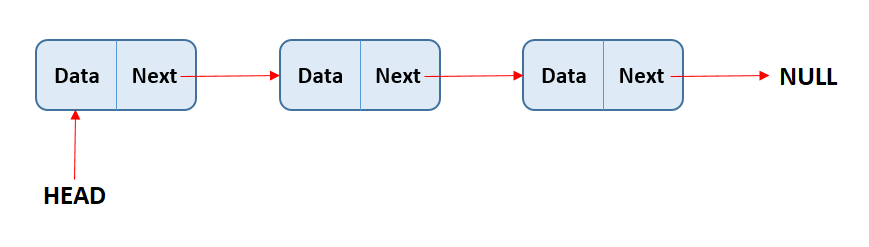
\includegraphics[scale=0.5]{linked-list.png}
\end{figure}
\subsubsection{Purpose of Head Node in Singly Linked List}
The Head Node in a Single Linked List is the most important node.
\begin{itemize}
	\item It points to the second node, which then points to the next node, and so on, essentially pointing to the entire linked list, which is scattered randomly in the memory.
	\item Losing the head node would mean losing the entire linked list.
	\item The head node is just a single node, and passing it around funtions makes it space efficient as opposed to passing the entire linked list or an entire array.
	\item The Head node being using just as a pointer to point to the entire linked list ensures that any function can perform any operation on the linked list by just taking the head node as a parameter.
\end{itemize}
\subsection{Various Operations on a Singly Linked List}
A \textit{Single Linked List} being an Abstract Data Type, has a variety of operations that you can perform on it, like:
\begin{enumerate}
	\item Searching: Look for a particular element with some key data in the entire linked list by traversing through it.
	\item Sorting: Sorting elements of a linked list just like any other data strucutre.
	\item Deleting: Deleting any element of the linked list by traversing through it.
	\item Inserting: Inserting an element at a given position in the linked lits.
	\item Merging: Merging 2 Linked lists in any way desirable, be it by merging their tails to the heads, or by creating copies of both the linked lists, and then returning the head of the copy.
	\item Displaing, etc.
\end{enumerate}

The Pseudo Codes for these functions are written further in the paper.
\section{Platform}
\textbf{Operating System}: Arch Linux x86-64 \\
\textbf{IDEs or Text Editors Used}: Visual Studio Code\\
\textbf{Compilers} : gcc on linux for C\\

\section{Input}

\begin{itemize}
	\item Atleast 5 Elements to Input, including the President and the Secretary
	\item Details of Every Element like Name and PRN
	\item Options to Select what to do.
\end{itemize}

\section{Output}
\begin{itemize}
	\item Menu to display all the operations you can perform on the Linked list.
	\item Display of All the elements of the Linked list, before and after performing operations on it.
\end{itemize}

\section{Test Conditions}
\begin{enumerate}
	\item Input at least 5 records.
	\item Inserting an Element at All Positions
	\item Delete an Element from All positions
\end{enumerate}

\section{Code}
\subsection{Pseudo Code}
\subsubsection{Pseudo Code for Creatoin of a Singly Linked List}
\begin{lstlisting}[language=C]
	struct node *head, *merged_head;
	head = (struct node *)malloc(sizeof(struct node));
	head->next = NULL;
	// then add new nodes. 
	struct node *temp = head;
	while(enter elements)
		struct node *curr = (struct node *)malloc(sizeof(struct node));
		scanf("%s", curr->Data);
		curr->next = NULL;
		temp->next = curr;
		temp = curr;
\end{lstlisting}
\subsubsection{Pseudo Code for Display of a Singly Linked List}
\begin{lstlisting}[language=C]
    if (head->next == NULL)
        print("\nNo members");
        return -1;
    struct node *curr = (struct node *)malloc(sizeof(struct node));
    curr = head->next;
    while (curr != NULL)
        print("\n--Member: %d--", ++counter);
        print("\Data: %s", curr->data);
        curr = curr->next;
    printf("\n");
\end{lstlisting}
\subsubsection{Pseudo Code for Insertion in a Singly Linked List}
\begin{lstlisting}[language=C]
	struct node *curr = head;
    struct node *nnode = (struct node *)malloc(sizeof(struct node));
    print(Enter data)
	scan(pos)
    pos--;
    int total_length = findLength(head);
    if (pos > total_length + 1)
        printf("Data cant be inserted!\n");
        return 0;
    else
        while (curr != NULL && i < total_length)
            i++;
            curr = curr->next;
        nnode->next = curr->next;
        curr->next = nnode;
\end{lstlisting}
\subsubsection{Pseudo Code for Deletion in a Singly Linked List}
\begin{lstlisting}[language=C]
	if (head->next == NULL)
		print("list empty")
		return -1;
    struct node *prev = (struct node *)malloc(sizeof(struct node *));
    prev = head;
    int count = 1;
    struct node *curr = (struct node *)malloc(sizeof(struct node *));
    curr = head->next;

    int len = find_total_members(head);

    if (position > len)
        scanf("\nCant Delete data");
    else
        while (count < position && curr->next != NULL)
            count++;
            prev = curr;
            curr = curr->next;
    struct node *temp = (struct node *)malloc(sizeof(struct node *));

    temp = curr;
    prev->next = curr->next;
    curr->next = NULL;
    free(temp);
\end{lstlisting}
\subsubsection{Pseudo Code for Reversing of a Singly Linked List}
\begin{lstlisting}[language=C]
    struct node *current = head->next;
    struct node *prev = NULL, *future = NULL;
    while (current != NULL)
        future = current->next;
        current->next = prev;
        prev = current;
        current = future;
    head->next = prev;
\end{lstlisting}
\subsubsection{Pseudo Code for Sorting of a Singly Linked List}
\begin{lstlisting}[language=C]
	struct node *i = (struct node *)malloc(sizeof(struct node));
    struct node *j = (struct node *)malloc(sizeof(struct node));
    struct node temp;

    // bubble sorting
    for (i = head; i != NULL; i = i->next)
        for (j = i; j->next != NULL; j = j->next)
            if (j->prn > j->next->prn)
                temp.prn = j->prn;
                j->prn = j->next->prn;
                j->next->prn = temp.prn;
\end{lstlisting}
\subsubsection{Pseudo Code for Merging of 2 Singly Linked Lists}
\begin{lstlisting}[language=C]
	struct node *merged_head = (struct node *)malloc(sizeof(struct node));
    merged_head->next = NULL;
    if (head->next == NULL || head_2->next == NULL)
        printf("\nOne of the nodes is empty, so no point in merging!\n");
        return merged_head;

    struct node *temp_head, *temp_merged, *current;
    temp_head = head->next;

    temp_merged = (struct node *)malloc(sizeof(struct node));
    merged_head->next = temp_merged;
    while (temp_head != NULL)
        current = temp_merged;
        temp_merged->prn = temp_head->prn;

        temp_merged = (struct node *)malloc(sizeof(struct node));
        current->next = temp_merged;
        temp_head = temp_head->next;

    temp_head = head_2->next;
    while (temp_head != NULL)
        current = temp_merged;
        temp_merged->prn = temp_head->prn;

        temp_merged = (struct node *)malloc(sizeof(struct node));
        current->next = temp_merged;
        temp_head = temp_head->next;

    current->next = NULL;

    return merged_head;
\end{lstlisting}
\subsection{C Implementation of Problem Statement}

\lstinputlisting[language=C, caption=Main.Cpp]{../Programs/[Krishnaraj]_[FDS]_Assignment_5.c}

\subsection{Input and Output}
\lstinputlisting[caption=Output]{../Programs/[Krishnaraj]_[FDS]_Assignment_5_output.txt}

\section{Time Complexity}
The Time complexities for Each Opertion: 
\begin{enumerate}
	\item Creation of a Single Linked List: 
	$$O(1)$$
	\item Insertion a Node at the End of a Single Linked List: 
	$$O(1)$$
	\item Insertion a Node at A Random Position of a Single Linked List: 
	$$O(N), \Omega(1)$$
	\item Accessing a Node at A Random Position of a Single Linked List: 
	$$O(N), \Omega(1)$$
	\item Deletion of a Node at the End of a Single Linked List: 
	$$O(1)$$
	\item Deletion at a Random Position of a Single Linked List: 
	$$O(N), \Omega(1)$$
\end{enumerate}
\section{Conclusion}
Thus, implemented all the operations of an Abstract Data type like Inserting, Searching, Sorting, Deleting and Reversing on a Singly Linked List.

\section{FAQs}
\begin{enumerate}
	\item \textbf{Write an ADT for Singly Linked List.}\\
	      An Abstract Data Type has 4 Main Operations:
	      \begin{enumerate}
		      \item Pseudo Code for Insertion in a Singly Linked List
		            \begin{lstlisting}[language=C]
struct node *curr = head;
struct node *nnode = (struct node *)malloc(sizeof(struct node));
print(Enter data)
scan(pos)
pos--;
int total_length = findLength(head);
if (pos > total_length + 1)
	printf("Data cant be inserted!\n");
	return 0;
else
	while (curr != NULL && i < total_length)
		i++;
		curr = curr->next;
	nnode->next = curr->next;
	curr->next = nnode;
					\end{lstlisting}
								\item Pseudo Code for Deletion in a Singly Linked List
		            \begin{lstlisting}[language=C]
if (head->next == NULL)
	print("list empty")
	return -1;
struct node *prev = (struct node *)malloc(sizeof(struct node *));
prev = head;
int count = 1;
struct node *curr = (struct node *)malloc(sizeof(struct node *));
curr = head->next;

int len = find_total_members(head);

if (position > len)
	scanf("\nCant Delete data");
else
	while (count < position && curr->next != NULL)
		count++;
		prev = curr;
		curr = curr->next;
struct node *temp = (struct node *)malloc(sizeof(struct node *));

temp = curr;
prev->next = curr->next;
curr->next = NULL;
free(temp);
					\end{lstlisting}
		      \item Pseudo Code for Searching an Element in a Single Linked List
		            \begin{lstlisting}[language=C]
printf("\nEnter item which you want to search?\n");   
scanf("%d",&item);  
while (ptr!=NULL)  
	if(ptr->data == item)  
		printf("item found at location %d ",i+1);  
		flag=0;  
	else  
		flag=1;  
	i++;  
	ptr = ptr -> next;  
if(flag==1)  
	printf("Item not found\n");  
					\end{lstlisting}
		      \item Pseudo Code for Modifying an Element in a Single Linked List
		            \begin{lstlisting}[language=C]
printf("\nEnter item which you want to Modify?\n");   
scanf("%d",&item);  
printf("\nEnter Modified data?\n");   
scanf("%d",&data_new);  
while (ptr!=NULL)  
	if(ptr->data == item)  
		ptr->data = data_new;
		printf(item modified);  
		flag=0;  
	else  
		flag=1;  
	i++;  
	ptr = ptr -> next;  
if(flag==1)  
	printf("Item not found\n");  
					\end{lstlisting}
	      \end{enumerate}
	\item \textbf{What are the disadvantages of a Singly Linked List?}\\
\begin{enumerate}
	\item \textit{Memory usage}
	: More memory is required in the linked list as compared to an array. Because in a linked list, a pointer is also required to store the address of the next element and it requires extra memory for itself.
	\item \textit{Traversal:} In a Linked list traversal is more time-consuming as compared to an array. Direct access to an element is not possible in a linked list as in an array by index. For example, for accessing a node at position n, one has to traverse all the nodes before it.
	\item \textit{Reverse Traversing}: In a singly linked list reverse traversing is not possible, but in the case of a doubly-linked list, it can be possible as it contains a pointer to the previously connected nodes with each node. For performing this extra memory is required for the back pointer hence, there is a wastage of memory.
	\item \textit{Random Access}: Random access is not possible in a linked list due to its dynamic memory allocation.
	
\end{enumerate}
	\item \textbf{Applications of Singly Linked List.}\\
\begin{enumerate}
	\item Implementation of stacks and queues
	\item Implementation of graphs: Adjacency list representation of graphs is the most popular which uses a linked list to store adjacent vertices.
	\item Dynamic memory allocation: We use a linked list of free blocks.
	\item Maintaining a directory of names
	\item Performing arithmetic operations on long integers
	\item Manipulation of polynomials by storing constants in the node of the linked list
	\item representing sparse matrices
\end{enumerate}

\end{enumerate}
\end{document}